\documentclass{standalone}
\usepackage{tikz}
\usetikzlibrary{patterns, positioning}


\begin{document}
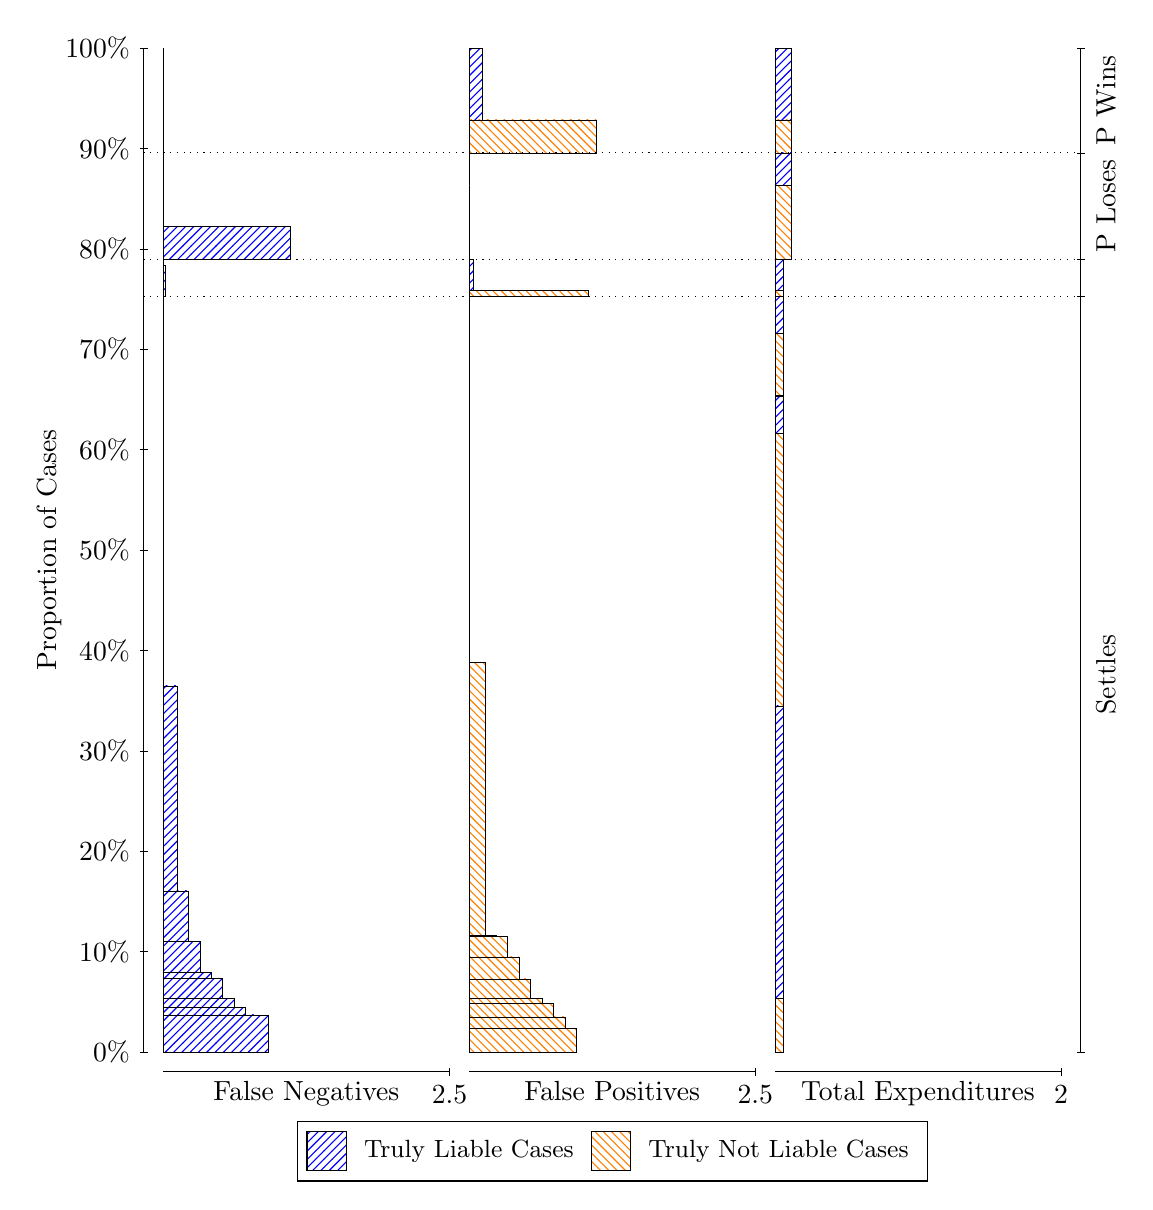
\begin{tikzpicture}
\draw[black, very thin] (1.5,1.75) -- (1.5,14.5);
\node[rotate=90, text=black, anchor=center] at (0.3, 8.125) {Proportion of Cases};
\draw[black, very thin] (1.45,1.75) -- (1.55,1.75);
\node[text=black, anchor=east] at (1.45, 1.75) {0\%};
\draw[black, very thin] (1.45,3.025) -- (1.55,3.025);
\node[text=black, anchor=east] at (1.45, 3.025) {10\%};
\draw[black, very thin] (1.45,4.3) -- (1.55,4.3);
\node[text=black, anchor=east] at (1.45, 4.3) {20\%};
\draw[black, very thin] (1.45,5.575) -- (1.55,5.575);
\node[text=black, anchor=east] at (1.45, 5.575) {30\%};
\draw[black, very thin] (1.45,6.85) -- (1.55,6.85);
\node[text=black, anchor=east] at (1.45, 6.85) {40\%};
\draw[black, very thin] (1.45,8.125) -- (1.55,8.125);
\node[text=black, anchor=east] at (1.45, 8.125) {50\%};
\draw[black, very thin] (1.45,9.4) -- (1.55,9.4);
\node[text=black, anchor=east] at (1.45, 9.4) {60\%};
\draw[black, very thin] (1.45,10.675) -- (1.55,10.675);
\node[text=black, anchor=east] at (1.45, 10.675) {70\%};
\draw[black, very thin] (1.45,11.95) -- (1.55,11.95);
\node[text=black, anchor=east] at (1.45, 11.95) {80\%};
\draw[black, very thin] (1.45,13.225) -- (1.55,13.225);
\node[text=black, anchor=east] at (1.45, 13.225) {90\%};
\draw[black, very thin] (1.45,14.5) -- (1.55,14.5);
\node[text=black, anchor=east] at (1.45, 14.5) {100\%};

\draw[black, very thin] (13.4,1.75) -- (13.4,14.5);
\draw[black, very thin] (13.35,1.75) -- (13.45,1.75);
\node[anchor=west] at (13.35, 1.75) {};
\draw[black, very thin] (13.35,11.342) -- (13.45,11.342);
\node[anchor=west] at (13.35, 11.342) {};
\draw[black, very thin] (13.35,11.814) -- (13.45,11.814);
\node[anchor=west] at (13.35, 11.814) {};
\draw[black, very thin] (13.35,13.169) -- (13.45,13.169);
\node[anchor=west] at (13.35, 13.169) {};
\draw[black, very thin] (13.35,14.5) -- (13.45,14.5);
\node[anchor=west] at (13.35, 14.5) {};

\draw[black, very thin, pattern color=blue, pattern=north east lines] (1.75,1.75) rectangle (3.0852,2.2143);
\draw[black, very thin, pattern color=blue, pattern=north east lines] (1.75,2.2143) rectangle (2.9399,2.2215);
\draw[black, very thin, pattern color=blue, pattern=north east lines] (1.75,2.2215) rectangle (2.7946,2.3168);
\draw[black, very thin, pattern color=blue, pattern=north east lines] (1.75,2.3168) rectangle (2.6492,2.4258);
\draw[black, very thin, pattern color=blue, pattern=north east lines] (1.75,2.4258) rectangle (2.5039,2.6851);
\draw[black, very thin, pattern color=blue, pattern=north east lines] (1.75,2.6851) rectangle (2.3586,2.759);
\draw[black, very thin, pattern color=blue, pattern=north east lines] (1.75,2.759) rectangle (2.2133,3.1576);
\draw[black, very thin, pattern color=blue, pattern=north east lines] (1.75,3.1576) rectangle (2.0679,3.7956);
\draw[black, very thin, pattern color=blue, pattern=north east lines] (1.75,3.7956) rectangle (1.9226,6.3982);
\draw[black, very thin, pattern color=orange, pattern=north west lines] (1.75,6.3982) rectangle (1.75,11.342);
\draw[black, very thin, pattern color=blue, pattern=north east lines] (1.75,11.342) rectangle (1.7773,11.737);
\draw[black, very thin, pattern color=orange, pattern=north west lines] (1.75,11.737) rectangle (1.75,11.814);
\draw[black, very thin, pattern color=blue, pattern=north east lines] (1.75,11.814) rectangle (3.3668,12.231);
\draw[black, very thin, pattern color=orange, pattern=north west lines] (1.75,12.231) rectangle (1.75,13.169);
\draw[black, very thin, pattern color=orange, pattern=north west lines] (1.75,13.169) rectangle (1.75,13.586);
\draw[black, very thin, pattern color=blue, pattern=north east lines] (1.75,13.586) rectangle (1.75,14.5);
\draw[black, very thin, pattern color=orange, pattern=north west lines] (5.6333,1.75) rectangle (6.9958,2.0532);
\draw[black, very thin, pattern color=orange, pattern=north west lines] (5.6333,2.0532) rectangle (6.8505,2.1956);
\draw[black, very thin, pattern color=orange, pattern=north west lines] (5.6333,2.1956) rectangle (6.7052,2.3682);
\draw[black, very thin, pattern color=orange, pattern=north west lines] (5.6333,2.3682) rectangle (6.5598,2.4313);
\draw[black, very thin, pattern color=orange, pattern=north west lines] (5.6333,2.4313) rectangle (6.4145,2.6777);
\draw[black, very thin, pattern color=orange, pattern=north west lines] (5.6333,2.6777) rectangle (6.2692,2.9575);
\draw[black, very thin, pattern color=orange, pattern=north west lines] (5.6333,2.9575) rectangle (6.1238,3.2171);
\draw[black, very thin, pattern color=orange, pattern=north west lines] (5.6333,3.2171) rectangle (5.9785,3.2259);
\draw[black, very thin, pattern color=orange, pattern=north west lines] (5.6333,3.2259) rectangle (5.8332,6.6936);
\draw[black, very thin, pattern color=blue, pattern=north east lines] (5.6333,6.6936) rectangle (5.6333,11.342);
\draw[black, very thin, pattern color=orange, pattern=north west lines] (5.6333,11.342) rectangle (7.1412,11.418);
\draw[black, very thin, pattern color=blue, pattern=north east lines] (5.6333,11.418) rectangle (5.6878,11.814);
\draw[black, very thin, pattern color=orange, pattern=north west lines] (5.6333,11.814) rectangle (5.6333,12.752);
\draw[black, very thin, pattern color=blue, pattern=north east lines] (5.6333,12.752) rectangle (5.6333,13.169);
\draw[black, very thin, pattern color=orange, pattern=north west lines] (5.6333,13.169) rectangle (7.2502,13.586);
\draw[black, very thin, pattern color=blue, pattern=north east lines] (5.6333,13.586) rectangle (5.7968,14.5);
\draw[black, very thin, pattern color=orange, pattern=north west lines] (9.5167,1.75) rectangle (9.6189,2.4313);
\draw[black, very thin, pattern color=blue, pattern=north east lines] (9.5167,2.4313) rectangle (9.6189,6.1444);
\draw[black, very thin, pattern color=orange, pattern=north west lines] (9.5167,6.1444) rectangle (9.6189,9.612);
\draw[black, very thin, pattern color=blue, pattern=north east lines] (9.5167,9.612) rectangle (9.6189,10.076);
\draw[black, very thin, pattern color=orange, pattern=north west lines] (9.5167,10.076) rectangle (9.6189,10.085);
\draw[black, very thin, pattern color=blue, pattern=north east lines] (9.5167,10.085) rectangle (9.6189,10.092);
\draw[black, very thin, pattern color=orange, pattern=north west lines] (9.5167,10.092) rectangle (9.6189,10.878);
\draw[black, very thin, pattern color=blue, pattern=north east lines] (9.5167,10.878) rectangle (9.6189,11.342);
\draw[black, very thin, pattern color=orange, pattern=north west lines] (9.5167,11.342) rectangle (9.6189,11.418);
\draw[black, very thin, pattern color=blue, pattern=north east lines] (9.5167,11.418) rectangle (9.6189,11.814);
\draw[black, very thin, pattern color=orange, pattern=north west lines] (9.5167,11.814) rectangle (9.721,12.752);
\draw[black, very thin, pattern color=blue, pattern=north east lines] (9.5167,12.752) rectangle (9.721,13.169);
\draw[black, very thin, pattern color=orange, pattern=north west lines] (9.5167,13.169) rectangle (9.721,13.586);
\draw[black, very thin, pattern color=blue, pattern=north east lines] (9.5167,13.586) rectangle (9.721,14.5);
\draw[black, dotted] (1.5,11.342) -- (13.4,11.342);
\draw[black, dotted] (1.5,11.814) -- (13.4,11.814);
\draw[black, dotted] (1.5,13.169) -- (13.4,13.169);
\draw[black, very thin] (1.75,1.5) -- (5.3833,1.5);
\node[text=black, anchor=north] at (3.5667, 1.5) {False Negatives};
\draw[black, very thin] (5.3833,1.45) -- (5.3833,1.55);
\node[text=black, anchor=north] at (5.3833, 1.45) {2.5};

\draw[black, very thin] (5.6333,1.5) -- (9.2667,1.5);
\node[text=black, anchor=north] at (7.45, 1.5) {False Positives};
\draw[black, very thin] (9.2667,1.45) -- (9.2667,1.55);
\node[text=black, anchor=north] at (9.2667, 1.45) {2.5};

\draw[black, very thin] (9.5167,1.5) -- (13.15,1.5);
\node[text=black, anchor=north] at (11.333, 1.5) {Total Expenditures};
\draw[black, very thin] (13.15,1.45) -- (13.15,1.55);
\node[text=black, anchor=north] at (13.15, 1.45) {2};

\node[text=black, centered, rotate=90] at (13.72, 6.5459) {Settles};

\node[text=black, centered, rotate=90] at (13.72, 12.492) {P Loses};
\node[text=black, centered, rotate=90] at (13.72, 13.834) {P Wins};

\draw (7.449999999999999,1.5) node[draw=none] (baseCoordinate) {};
\begin{scope}[align=center]
        \matrix[scale=0.5, draw=black, below=0.5cm of baseCoordinate, nodes={draw}, column sep=0.1cm]{
            \node[rectangle, draw, minimum width=0.5cm, minimum height=0.5cm, pattern color=blue, pattern=north east lines] {}; &
            \node[draw=none, font=\small, text=black] (B) {Truly Liable Cases}; &
            \node[rectangle, draw, minimum width=0.5cm, minimum height=0.5cm, pattern color=orange, pattern=north west lines] {}; &
            \node[draw=none, font=\small, text=black] (B) {Truly Not Liable Cases}; \\
            };
\end{scope}

\end{tikzpicture}
\end{document}